% !TeX encoding = UTF-8

\documentclass{protokol}

\usepackage{pdfpages}
\usepackage{tikz}
\usetikzlibrary{calc}
\usetikzlibrary{arrows}

%====== Units =====
\usepackage{siunitx}
\sisetup{inter-unit-product =\ensuremath{\cdot}}
\sisetup{group-digits = integer}
\sisetup{output-decimal-marker = {,}}
\sisetup{exponent-product = \ensuremath{\cdot}}
\sisetup{separate-uncertainty}
\sisetup{tight-spacing = false}
%\sisetup{scientific-notation = true}
%\sisetup{round-mode=places,round-precision=4}
%\sisetup{evaluate-expression}


%====== Grafy =====
\usepackage{pgfplots}
\pgfplotsset{width=0.8\linewidth, compat=1.17}
\def\plotcscale{0.8}
\usepackage{pgfplotstable}
\usepackage[figurename=Obr.]{caption} % figure caption rename

%====== Rovnice align block ======
\usepackage{amsmath}
\setlength{\jot}{10pt} % rozestup mezi řádky

\graphicspath{ {./img/} }

%====== Vyplňte údaje ======
\jmeno{Jakub Charvot}
\kod{240844}
\rocnik{3.}
\obor{MET}
\skupina{MET/2}
\spolupracoval{Radek Kučera}

\merenodne{26.03.\ 2024}
\odevzdanodne{02.03.\ 2024}
\nazev{Měření polohy}
\cislo{1} %měřené úlohy

\predmet{Mikrosenzory a mikromechanické systémy}
\ustav{Ústav mikroelektroniky}
\skola{FEKT VUT v~Brně}

\def\para{x+0}
\def\parb{\para-80}


% %citace 
% \usepackage[backend=biber, style=iso-numeric, sortlocale=cs_CZ, autolang=other, language=czech]{biblatex}
% \addbibresource{bibliography.bib}
% \DeclareFieldFormat{labelnumberwidth}{\mkbibbrackets{#1}}
% hyperlinky
\usepackage[colorlinks]{hyperref}

% odstavce
\usepackage{parskip}

% Bloky kódu
\usepackage{xcolor}

%New colors defined below
\definecolor{codegreen}{rgb}{0,0.6,0}
\definecolor{codegray}{rgb}{0.5,0.5,0.5}
\definecolor{codepurple}{rgb}{0.58,0,0.82}
\definecolor{backcolour}{rgb}{0.95,0.95,0.92}

\usepackage{listings}
\lstdefinestyle{mystyle}{
  backgroundcolor=\color{backcolour}, commentstyle=\color{codegreen},
  keywordstyle=\color{magenta},
  numberstyle=\tiny\color{codegray},
  stringstyle=\color{codepurple},
  basicstyle=\ttfamily\footnotesize,
  breakatwhitespace=false,         
  breaklines=true,                 
  captionpos=b,                    
  keepspaces=true,                 
  numbers=left,                    
  numbersep=5pt,                  
  showspaces=false,                
  showstringspaces=false,
  showtabs=false,                  
  tabsize=2
}
\lstset{
	inputencoding=utf8,
	extendedchars=true,
	literate={á}{{\'a}}1 {č}{{\v{c}}}1 {ď}{{\v{d}}}1 {é}{{\'e}}1 {ě}{{\v{e}}}1 
           {í}{{\'i}}1 {ň}{{\v{n}}}1 {ó}{{\'o}}1 {ř}{{\v{r}}}1 {š}{{\v{s}}}1 
           {ť}{{\v{t}}}1 {ú}{{\'u}}1 {ů}{{\r{u}}}1 {ý}{{\'y}}1 {ž}{{\v{z}}}1 
           {Á}{{\'A}}1 {Č}{{\v{C}}}1 {Ď}{{\v{D}}}1 {É}{{\'E}}1 {Ě}{{\v{E}}}1 
           {Í}{{\'I}}1 {Ň}{{\v{N}}}1 {Ó}{{\'O}}1 {Ř}{{\v{R}}}1 {Š}{{\v{S}}}1 
           {Ť}{{\v{T}}}1 {Ú}{{\'U}}1 {Ů}{{\r{U}}}1 {Ý}{{\'Y}}1 {Ž}{{\v{Z}}}1,
	style=mystyle
	}

% Číslování
\pagenumbering{arabic}

% Tabulky
\usepackage{booktabs}

% =========================================
% =============== DOKUMENT ================
% =========================================
\begin{document}
	%====== Vygenerování tabulky ======a
    \maketitle

    \section{Měření a jeho vyhodnocení }

    \begin{table}[ht!]
        \caption{ Hodnoty naměřené při kalibraci měření.}
        \def\arraystretch{1.2}
        \centering
        \begin{tabular}{lrrrrr}
            \toprule
            l [cm] & 10 & 20 & 30 & 40 & 50 \\
            t [ms] & 0,54 & 1,08 & 1,68 & 2,22 & 2,82 \\
            \bottomrule
        \end{tabular}
    \end{table}

    \begin{table}[ht!]
        \caption{ Naměřené a vypočítané hodnoty vlnovodu.}
        \def\arraystretch{1.2}
        \centering
        \begin{tabular}{rrr}
            \toprule
            t [ms] & $l_{VYP}$  [\unit{{m}}] &  $l_{MER} $[\unit{{m}}] \\
            \midrule
            5,40 & 1,90 & 1,87 \\
            \bottomrule
            \end{tabular}
    \end{table}



    \begin{table}[ht!]
        \caption{Hodnoty odrazivosti materiálů (\(l=\qty{30}{cm}\) ).}
        \def\arraystretch{1.2}
        \centering
        \begin{tabular}{lrrr}
\toprule
Materiál & $\alpha [\unit{{\degree}}]$ & $U_{{max}}$ [\unit{{\mV}}] & R [\unit{{\percent}}] \\
\midrule
Pevná deska & 0,00 & 583,00 & 100,00 \\
Pevná deska & 22,50 & 307,00 & 52,66 \\
Pevná deska & 45,00 & 61,00 & 10,46 \\
Pevná deska & 67,50 & 61,00 & 10,46 \\
Lisovaná akustická pěna & 0,00 & 58,00 & 9,95 \\
Lisovaná akustická pěna & 22,50 & 63,00 & 10,81 \\
Lisovaná akustická pěna & 45,00 & 58,00 & 9,95 \\
Lisovaná akustická pěna & 67,50 & 53,00 & 9,09 \\
Profilovaná akustická pěna -- trojúhelník & 0,00 & 58,00 & 9,95 \\
Profilovaná akustická pěna -- trojúhelník & 22,50 & 56,00 & 9,61 \\
Profilovaná akustická pěna -- trojúhelník & 45,00 & 61,00 & 10,46 \\
Profilovaná akustická pěna -- trojúhelník & 67,50 & 61,00 & 10,46 \\
\bottomrule
\end{tabular}

    \end{table}

    \begin{figure}[h!]
        \centering
        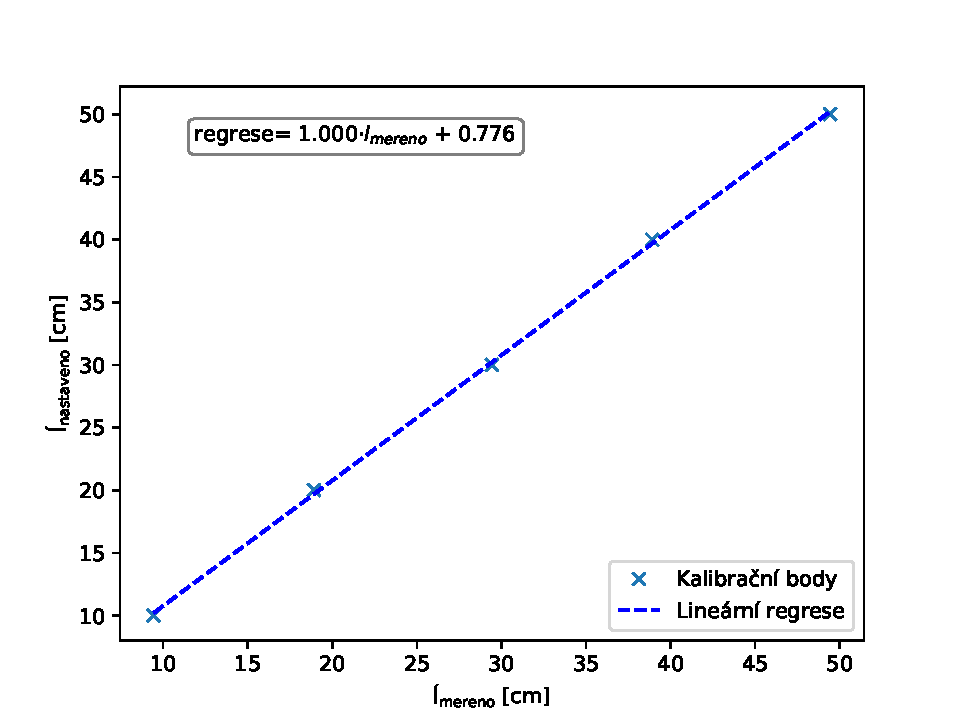
\includegraphics[width=0.8\textwidth]{img/graf2.pdf}
        \caption{Kalibrační křivka dálkoměru.}
        \label{fig:img/graf-2}
    \end{figure}

    % \begin{figure}[h!]
    %     \centering
    %     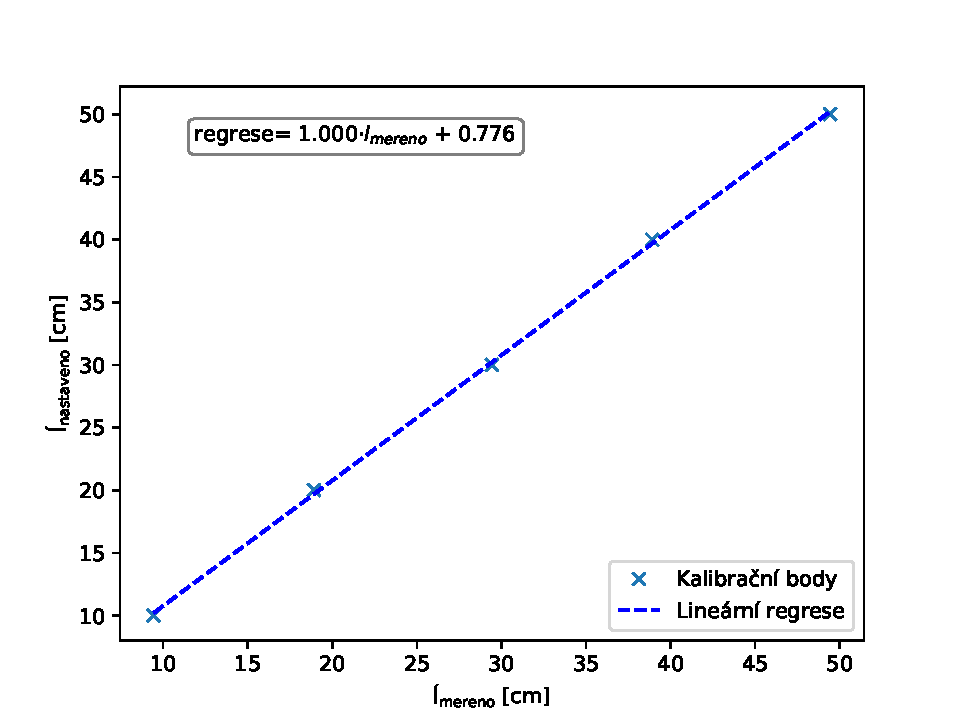
\includegraphics[width=0.8\textwidth]{img/graf2.pdf}
    %     \caption{Závislost vypočítaného tlaku na referenčním tlaku.}
    %     \label{fig:img/graf-2}
    % \end{figure}

    \begin{figure}[h!]
        \centering
        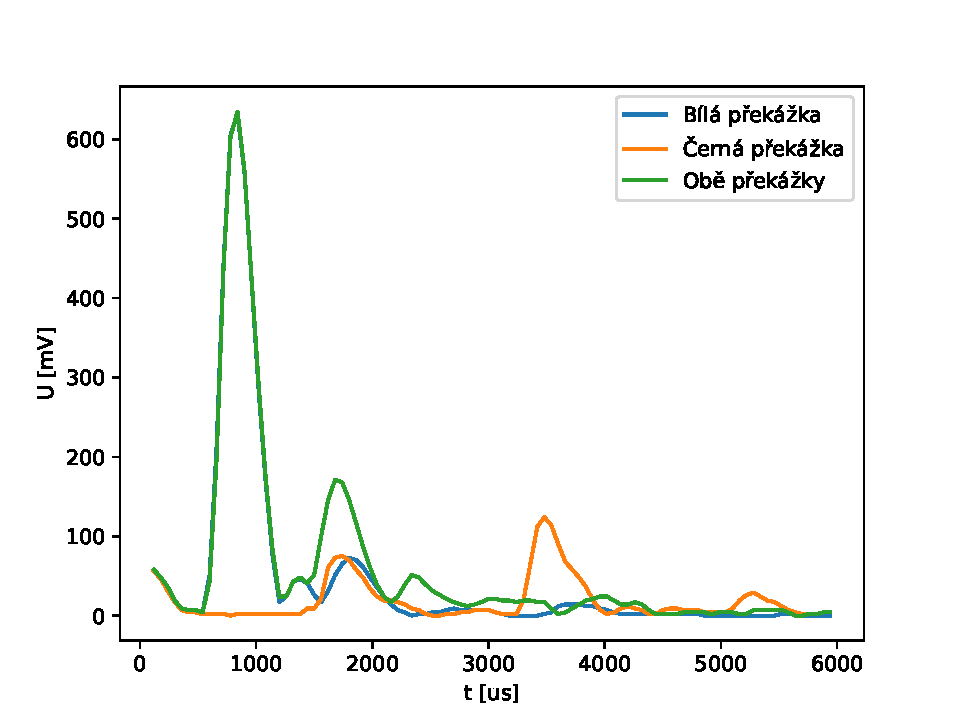
\includegraphics[width=0.8\textwidth]{img/graf3.pdf}
        \caption{Průběhy měření vzdálenosti dvou předmětů.}
        \label{fig:img/graf-3}
    \end{figure}

    \begin{figure}[h!]
        \centering
        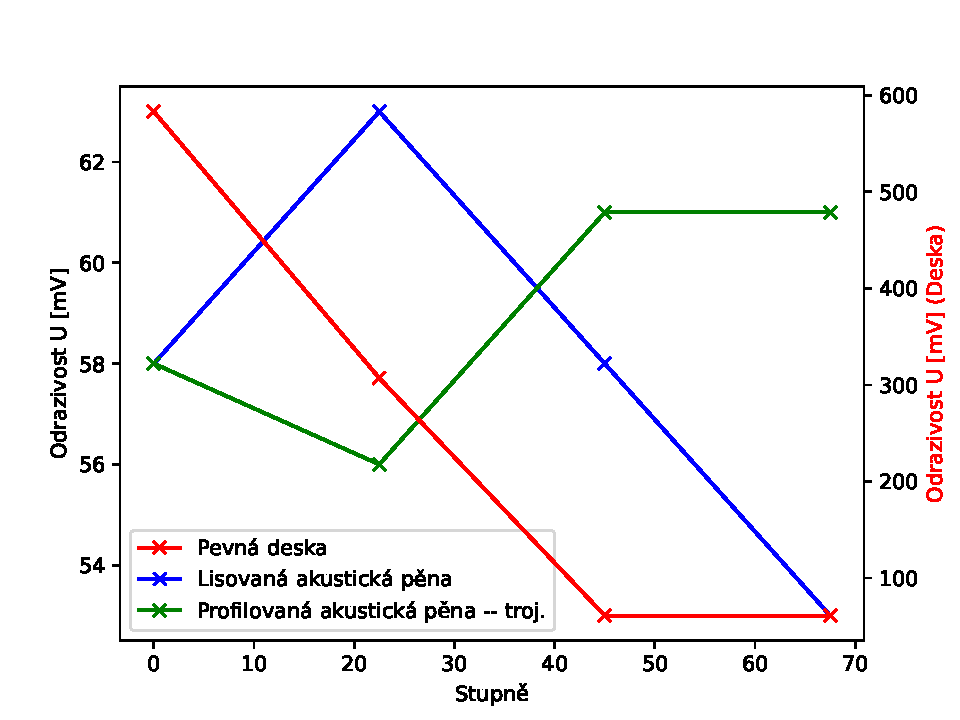
\includegraphics[width=0.8\textwidth]{img/graf4.pdf}
        \caption{Závislost odrazivosti na úhlu a materiálu reflektoru.}
        \label{fig:img/graf-4}
    \end{figure}

    \subsection{Příklad výpočtu}
        Výpočet délky vlnovodu:
        \begin{align*}
            l_{VYP} =& v \cdot t  \\
            l_{VYP} =& \num{331.6}+\theta\cdot \num{0.61} \cdot t  \\
            l_{VYP} =& \num{331.6}+\num{32}\cdot \num{0.61} \cdot \num{5400e-6}  \\
            l_{VYP} =& \qty{1,8986832}{m} 
        \end{align*}
        kde \(v\) je rychlost zvuku ve vzduchu, \(\theta\) je teplota vzduchu (GIEMZA) a \(t\) je čas k naměření maxima napětí (GIEMZA).

        Příklad výpočtu odrazivosti materiálu pro druhý řádek tabulky:
        \begin{align*}
            R =& \frac{U_{max}}{U_{max-ref}}\cdot  100  \\
            R =& \frac{\num{307}}{583}\cdot  100  \\
            R =& \qty{52,66}{\percent}  \\
        \end{align*}
        Jako referenční je použita pevná deska (první řádek tabulky).

        Rovnice regrese kalibrační křivky byla vypočtena za pomoci pythonu, který využívá metodu nejmenších čtverců.

        
        
        \clearpage
        \section*{Závěr}
            V této úloze jsme kalibrovali ultrazvukový dálkoměr. Jak je vidět z kalibrační křivky na Obr. 1, senzor měří na zvoleném rozsahu poměrně přesně.
            
            Z fyzikální podstata šíření vln vyplývá, že intenzita signálu (zde zvuku) klesá se čtvercem vzdálenosti. Ačkoliv graf pro tyto hodnoty nebyl v úloze požadován, byl vytvořen a zmíněný trend poklesu byl potvrzen, z důvody úspory papíru ovšem není graf přiložen.
            
            Při měření části úlohy se dvěma překážkami pravděpodobně došlo buďto k chybě měření nebo k neúmyslné záměně měřených dat, protože průběhy pro měření samostatných překážek neodpovídají svým tvarem předchozím měřením, popis situace na grafu je tedy poněkud obtížný. Pro případ obou překážek se zdá, že byla zachycena pouze překážka bližší, pokud však byla umístěna samostatně, zachycena nebyla (resp. peak neodpovídá vzdálenosti).
\end{document}
